% !TEX root = thesis.tex
\renewcommand{\figurename}{Figura}
\renewcommand{\proofname}{Demostració}
\newtheorem{definition}{Definició}
\newtheorem{theorem}{Teorema}
\newtheorem{proposition}{Proposició}
\newtheorem{corolary}{Corol·lari}
\newtheorem{lemma}{Lema}

\section{Introducció}\label{sec:Introducció}
L'espècie humana té coneixement dels nusos desde temps prehistòrics. Començant per l'enregistrament d'informació, les xarxes de pesca o fins i tot per motius religiosos, els nusos han estat de gran importància per la seva utilitat i simbologia espiritual. Moltes obres d'art de cultures d'arreu del món presenten aquestes figures en les seves obres. Alguns exemples son la cultura Xinesa, Tibetana o Celta.\\

Els nusos comencen a tenir la seva presència dins el món de les matemàtiques a partir de l'any 1771 degut als treballs realitzats per Alexandre-Théophile Vandermonde el qual es dedicà a estudiar les propietats topològiques dels nusos en relació a la seva posició en l'espai. Treballs posteriors de Carl Friedrich Gau\ss$ $ qui va definir diverses propietats d'aquests objectes [\cite{knottheory}] van projectar aquesta teoria a la fama. L'any 1860 la teoria sobre l'atom en l'aether formulada per William Thomson va dur a Peter Guthrie Tait a la creació de les primeres taules de nusos. L'any 1885, aquest va publicar la primera taula amb tots els nusos de fins a deu creuaments, també va formular les conjectures que duen el seu nom.\\

A principis del segle XX, Max Dehn i J. W. Alexander van estudiar els nusos des del punt de vista de la teoria de grups i el seus invariants utilitzant grups d'homologia, cosa que va dur a la creació d'un dels primers invariants algebràics de la teoria, el polinomi d'Alexander.\\

A finals de l'any 1970, la incorporació de la geometria hiperbòlica en l'estudi dels nusos utilitzant el teorema de Geometrització de Thurston va permetre classificar aquests en funció de la seva mètrica, permetent l'ús de la geometria en la creació de nous invariants. El descobriment del polinomi de Jones per part de Vaughan Jones l'any 1984 [\cite{mathwithatwist}] juntament amb contribucions de Edward Witten i Maxim Kontsevich van revelar fortes relacions entre la teoria de nusos i mètodes matemàtics en mecànica estadística i teoria quàntica de camps. Una gran quantitat de invariant han estat inventats desde llavors utilitzant eines com els grups quàntics o la homologia de Floer.\\

En les darreres dècades, els científics han estat interessats en l'estudi dels nusos físics per tal de comprendre el nuament de l'ADN i de diferents polímers. Aquesta teoria s'utilitza també per determinar si una molècula és o no quiral. Finalment, la teoria de nusos pot ser crucial en la construcció dels primers ordinadors quàntics a través del model proposat per Alexei Kitaev [\cite{computingwithquantumknots}].\\

\subsection{Sobre els nusos}\label{subsec:sobreelsnusos}
Els nusos, son estructures presents en el nostre dia a dia. La Figura \ref{fig:exemples de nusos} mostra un parell d'exemples del que considerem nus en el sentit habitual.\\

\begin{figure}
  \centering
  \includegraphics[width=0.46\linewidth]{img/nus simple.jpg}
  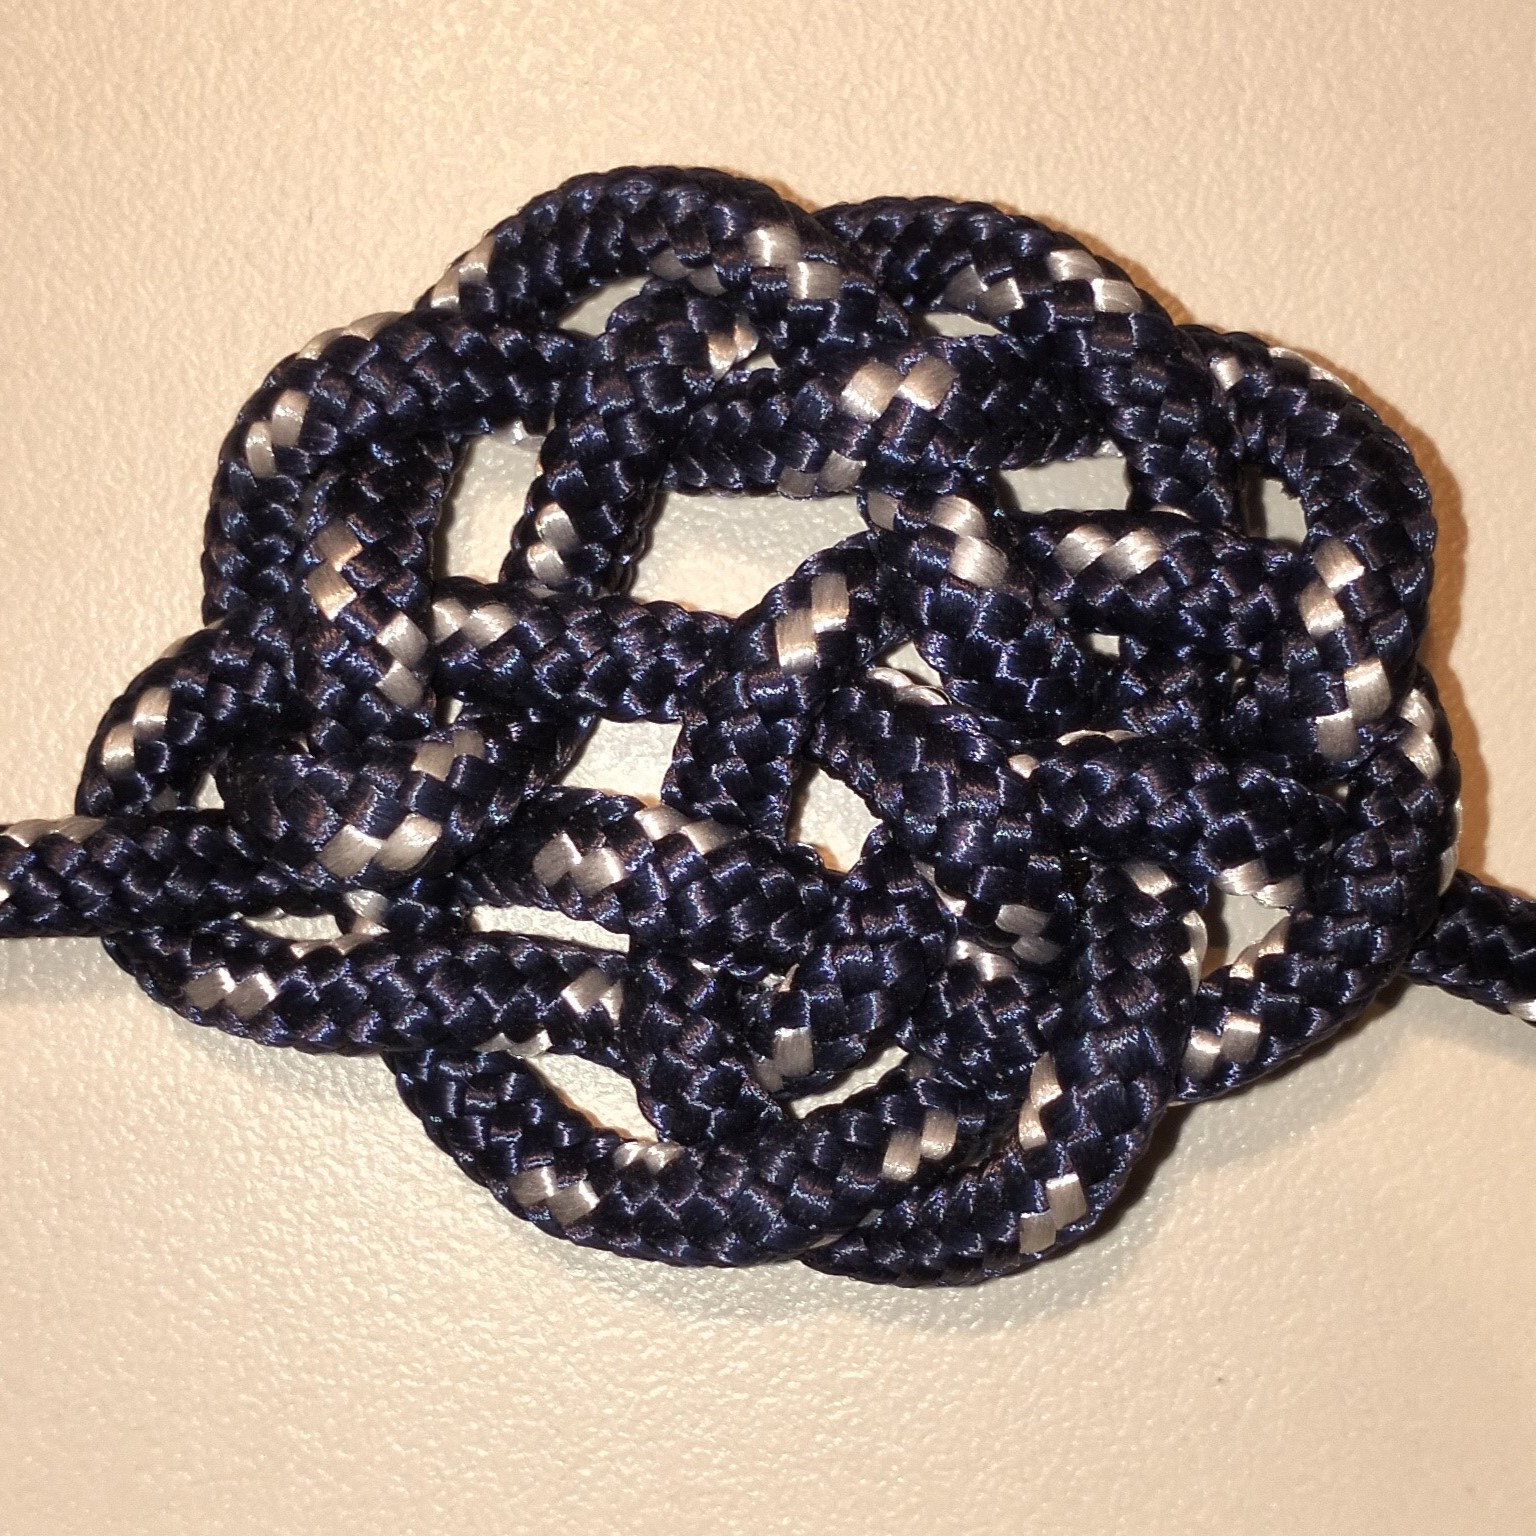
\includegraphics[width=0.46\linewidth]{img/arbre de la vida.jpg}
  \caption{D'esquerra a dreta: Nus simple (Overhand Knot en anglès) i Arbre de la vida, nus celta símbol de la naturalesa.
  }\label{fig:exemples de nusos}
\end{figure}

El problema que tenen aquests nusos és que, aquests mantenen la seva forma a partir de la tensió i fricció que existeix entre les cordes que formen el nus. No és gaire difícil veure que un podria desfer aquests nusos de manera que acabariem obtenint una simple corda sense cap nus. És per això, que en matemàtiques és necessari considerar una definició més restrictiva d'aquest concepte per tal de preservar-ne l'estructura. Podriem pensar, que si uníssim els caps de les cordes de la Figura \ref{fig:exemples de nusos}, aleshores només tallant la corda seriem capaços de desfer el nus (això precisa de demostració!).